
\setcounter{page}{1}


\documentclass[hidelinks, 11pt]{article}

\usepackage{amsmath,amsfonts,amssymb, dsfont}
\usepackage{tabularx,color,colortbl}
\usepackage{graphicx}
\usepackage{subcaption}
\usepackage{booktabs}
%\usepackage{enumitem}
\usepackage{pdflscape}
\usepackage{float}
%\usepackage{dsfont}
\usepackage{nameref}
%\usepackage[hidelinks]{hyperref}																					
%\hypersetup{colorlinks, citecolor=blue, linkcolor=black, urlcolor=blue}
\usepackage[longnamesfirst]{natbib}
%\usepackage{enumitem}
%\usepackage[pdftex]{hyperref}


% Select what to do with todonotes:
%\usepackage[disable]{todonotes} % notes not showed
%\usepackage[draft]{todonotes}   % notes showed

\usepackage{verbatim}
\usepackage{rotating}

%\usepackage{comment}\excludecomment{hide}

\newcommand{\E}{\mathbb{E}}
\newcommand{\var}{\mathrm{Var}}
\newcommand{\p}{\mathbb{P}}
\newcommand{\one}{\mathbb{1}}
\newcommand{\f}{\mathcal{F}}
\newcommand{\cov}{\mathrm{Cov}}
\newcommand{\corr}{\mathrm{Corr}}
\newcommand{\R}{\mathbb{R}}
\newcommand{\K}{\mathbb{K}}
\newcommand{\N}{\mathcal{N}}
\newcommand\numberthis{\addtocounter{equation}{1}\tag{\theequation}}

%\usepackage{epigraph}
%\epigraphfontsize{\normalsize}
%\setlength\epigraphwidth{1\textwidth}
%\setlength\epigraphrule{0pt}


%%% NATEBIB "AND" between cites


\newcolumntype{C}{>{\centering\arraybackslash}X}

%\usepackage[top=3cm,bottom=3cm,left=2.5cm,right=3cm]{geometry}
\usepackage[top=1.49in,bottom=1.48in,left=1in,right=1in]{geometry}
%\usepackage[top=1.5in,bottom=1.5in,left=1in,right=1in]{geometry}
%\usepackage[font=bf]{caption}

%%% RFS Conventions %%%
% Section numbering under the JF should comment out
%\renewcommand{\@seccntformat}[1]{{\csname the#1\endcsname}.\hspace{0.5em}}

%%% Journal of Finance conventions %%%
%\renewcommand{\thesection}{\Roman{section}}
%\renewcommand{\thesubsection}{\Alph{subsection}}

%\renewcommand{\thetable}{\Roman{table}}
\renewcommand{\abstractname}{{\sc ABSTRACT}}
%\renewcommand\labelitemi{{\boldmath$\cdot$}}
\renewcommand\labelitemi{\raisebox{0.35ex}{\tiny$\bullet$}}

\makeatletter
% we need a period (.) after sectioning numbers, but not in cites thereto.


\long\def\@makefigcaption#1#2{%
	\vskip\abovecaptionskip
	\sbox\@tempboxa{\textbf{#1.} #2}%
	\ifdim \wd\@tempboxa >\hsize
	\textbf{#1.} #2\par
	\else
	\global \@minipagefalse
	\hb@xt@\hsize{\hfil\box\@tempboxa\hfil}%
	\fi
	\vskip\belowcaptionskip}

\renewcommand{\figure}{\let\@makecaption\@makefigcaption\@float{figure}}

\long\def\@maketblcaption#1#2{%
	\vskip\abovecaptionskip
	\begin{center}\small\bf#1\\\normalsize#2\end{center}
	\vskip\belowcaptionskip}

\renewcommand{\table}{\let\@makecaption\@maketblcaption\@float{table}}

\makeatother



\usepackage{setspace}
\usepackage{caption}
\usepackage{lscape,scalefnt,xspace}

\setcounter{MaxMatrixCols}{10}

\newcommand\T{\rule{0pt}{2.6ex}}
\newcommand\B{\rule[-1.2ex]{0pt}{0pt}}
\newcommand\TX{\rule{0pt}{3.6ex}}
\newcommand\BX{\rule[-2.2ex]{0pt}{0pt}}
\DeclareCaptionLabelFormat{figure-short}{}
\DeclareCaptionLabelFormat{table-short}{}

%\newcommand\comment[1]{\textcolor{red}{\emph{#1}}}
%\newcommand\olli[1]{\textcolor{blue}{\emph{#1}}}
\newcommand\str[1]{\textcolor{red}{\emph{\st{#1}}}}

% Hypothesis
%\usepackage{ntheorem}
%\newtheorem{hyp}{Hypothesis}

\makeatletter
\newcounter{subhyp}
\let\savedc@hyp\c@hyp
\newenvironment{subhyp}
{%
	\setcounter{subhyp}{0}%
	\stepcounter{hyp}%
	\edef\saved@hyp{\thehyp}% Save the current value of hyp
	\let\c@hyp\c@subhyp     % Now hyp is subhyp
	\renewcommand{\thehyp}{\saved@hyp\alph{hyp}}%
}
{}
\newcommand{\normhyp}{%
	\let\c@hyp\savedc@hyp % revert to the old one
	\renewcommand\thehyp{\arabic{hyp}}%
}
\makeatother

% BIBTEX
\bibpunct{(}{)}{,}{a}{,}{,}
%Included for Gather Purpose only:
%input "d:\00_MyFolder\Dropbox\SharedFolders\MF_BAB\paper\MFBAB.bib"


\interfootnotelinepenalty=10000

\def\papertitle{Robust microstructure: \#fincap}

% alternative title:  Price Revelation of Fundamentals from Insider Trading: Evidence from Hacked Earnings News

% Retail Traders and Market Price Efficiency: \\ Evidence from Hacked Earnings News

\begin{document}
%	
%\title{\papertitle }
%	
\title{	\vspace{-3.5em}\papertitle \vspace{-2em} }
%\author{{Vincent Gr\'egoire and Charles Martineau}\thanks{
%		Gr\'egoire: HEC Montr\'eal, 3000 Chemin de la C\^{o}te-Sainte-Catherine, Montr\'eal, QC H3T 2A7 (vincent.3.gregoire@hec.ca).
%		Martineau: University of Toronto, 105 St. George Street, Toronto ON, Canada, M5S 3E6 (charles.martineau@rotman.utoronto.ca).}
%}%$^\dagger$}
%\date{}



	%\author{}
	
	\maketitle
	
	\vspace{-4.5em}
%	\thispagestyle{empty}
%
%		
%	\begin{abstract}
%	%\input{abstract_v01}
%		
%		\bigskip
%		
%	%	\noindent \textit{JEL Classification}: G10, G12, G14 \\
%
%	%	\noindent \textit{Keywords}: cyber risks, earnings announcements, informed trading, liquidity, market microstructure, price discovery
%	\end{abstract}
%	
%	
%	\thispagestyle{empty} \newpage \setcounter{page}{1}
	\fontsize{12}{22}\selectfont
	
%\listoftodos  % remove the todo lists
%\clearpage
	

\section{Methodology}
%We examine how key microstructure measures changes over time. All our tests are based on changes in the log value of our measures. For each measure $Y$, we estimate the following regression on monthly observations:

To examine how key market microstructure measures changed between 2002 and 2018\footnote{For measures requiring signed trades, our sample period is Nov. 2009 to Dec. 2018.} for the EURO STOXX 50® Index Futures, we estimate the following regression using monthly observations:
\begin{equation}
log(Y_t) = \alpha + \beta X_t + \varepsilon_t,
\end{equation}
where $log(Y_t)$ is the log value of our measure and $X_t$ is a time variable equal to $1/12$ for the first observation and increasing by $1/12$ each month. The $\widehat{\beta}$ estimate can be interpreted as the per-year change in \%. We compute Heteroskedasticity and Autocorrelation-Consistent (HAC) standard errors with 6 lags. Figure \ref{fig:timeseriesmonthly} shows the time-series of each measures and Table \ref{tab:RegResults} reports our regression estimates.


\section{Results}
%\subsection{Market efficiency}
\subsection{Null hypothesis 1: Market efficiency has not changed over time.}

%Assuming that informationally-efficient prices follow a random walk, did market efficiency change over time?
%\begin{align*}
%p_{t}=p_{t-1}+\varepsilon_{t}& \Rightarrow p_{t}=p_{t-2}+\varepsilon
%_{t-1}+\varepsilon_{t}\\
%&\Rightarrow p_{t}-p_{t-n}=\sum_{i=1}^{n}\varepsilon_{t-i+1}%
%\end{align*}

If informationally-efficient log prices follow a random walk ($p_t=p_{t-1}+\varepsilon_{t} $) and assuming that $E\left(  \varepsilon_{t}\varepsilon_{t-j}\right)  =0$ $\forall j$, we have that $Var\left(  p_{t}-p_{t-n}\right) = n\sigma_{\varepsilon}^2$.

\noindent We define the Variance Ratio \citep{lo1988stock} as:
\begin{equation}
VR\left(n, k\right)  =\frac{kVar\left(  p_{t}-p_{t-n}\right)
}{nVar\left(  p_{t}-p_{t-k}\right)  }
\end{equation}

\noindent Under the null, prices follow a random walk, $VR\left(n, k\right)=1$. To test for \emph{changes} in market efficiency, we follow \cite{o2011market} and compute the absolute difference between 1 and $VR\left(n, k\right)$:
\begin{equation}
ABS\_VR\left(n, k\right)  = \left|1 - VR\left(n, k\right)\right|
\end{equation}

\noindent Low values of $ABS\_VR\left(n, k\right)$ are associated with an efficient market and prices behaving like a random walk.
Choices for $n$ and $k$ are up to the econometrician, and values used in the literature vary. For example, \cite{lo1988stock} use 2 to 8 weeks over 1 week while \cite{comerton2019inverted} use 1 minute over 15 seconds. In modern markets, choosing higher frequency measures is more reasonable. Variance ratios are estimated from midquote prices, but our data only contains trades. To mitigate issues from using trade prices \citep[see, e.g.][]{gregoire2020earnings}, we use  $n=$30 minutes and $k=$5 minutes, and only consider trades on the front-most contract.\footnote{We roll over to the next contract on the expiry date, we do not consider a contract on the day it expires.} We compute daily $ABS\_VR$s and then take the monthly average for our regressions. 

We do not reject the null of no change as our measure ABS\_VR increased by 0.531\% on average per year where the standard error of this change is 0.449\% and the resulting $t$-statistic is 1.182 ($p$-value is 0.237).

%\textbf{Null hypothesis 1: Market efficiency has not changed over time.}

%\subsection{Cost of trading}
\subsection{Null hypothesis 2: The realized spread on market orders has not changed over time.}\label{sec:cot}
%Did the (realized) bid-ask spread paid on market orders change over time?

%The realized spread could be thought of as the gross-profit component of the spread as earned by the limit-order submitter.

We define the realized spread as in \cite{goyenko2009liquidity}:
\begin{align}
REAL\_SPREAD(\Delta) &= \left\{
\begin{array}{ll}
2(p_{t} - m_{t+\Delta}) & \text{for buyer-initiated trades}, \\
2(m_{t+\Delta} - p_{t}) & \text{for seller-initiated trades},
\end{array}\right.
\end{align}
where $p_t$ is the log traded price for the transaction at time $t$, and $m_t$ is the prevailing log midquote at time $t$. Since our data only contains trade prices, we approximate $m_{t+\Delta}$ with the price of the last transaction at time $t+\Delta$. To mitigate issues associated with sparse trading, we use $\Delta=5$ minutes and only consider trades on the front-most contract. We estimate realized spread for individual trades and winsorize the top and bottom 0.5\% trades in each month. We thencompute the monthly realized spread as the quantity-weighted average for all trades in the month. %The sample begins later than for other tests because the trade direction is only available starting on Nov. 16, 2009.

%\textbf{Null hypothesis 2: The realized spread on market orders has not
%changed over time.}

We do not reject the null of no change as our measure REAL\_SPREAD declined by 1.534\% on average per year where the standard error of this change is 3.459\% and the resulting $t$-statistic is -0.444 ($p$-value is 0.657).


%\subsection{Client trades only}
%The remaining hypotheses focus on client trades only (i.e., trades implemented by exchange members on behalf of their clients).

%\subsubsection{Share of client volume}

%Did the share of client volume in total volume change over time?

\subsection{Null hypothesis 3: Client share volume as a fraction of total volume has not changed over time.}

We compute the monthly share of client volume in total volume using all trades for all maturities as:
\begin{equation}
SHR\_CLIENT\_VOL  = \frac{\sum_{n=1}^N q_n \times \mathds{1}_{n,\text{client}}}{\sum_{n=1}^N q_n }
\end{equation}
where $q_n$ is the quantity of trade $n$ and $\mathds{1}_{n,\text{client}}$ is an indicator variable equal to one if trade $n$ is a client trade and zero otherwise.

%\textbf{Null hypothesis 3: Client share volume as a fraction of total
%volume has not changed over time.}

We reject the null of no change. We find that the share of client volume in total volume declined as our measure SHR\_CLIENT\_VOL declined by 3.723\% on average per year where the standard error of this change is 0.270\% and the resulting $t$-statistic is -13.812 ($p$-value is $<$ 0.001). 

This result shows that client trades make up a much smaller fraction of total volume than they did 20 years ago. This is consistent with our observations from Panel C of Figure \ref{fig:timeseriesmonthly} showing a gradual decrease over the sample period with a sharp decrease around the GFC.


%\subsubsection{Cost of trading for client trades}\label{sec:cot_clients}
\subsection{Null hypothesis 4: Client realized spreads have not changed over time.}\label{sec:cot_clients}

%On their market orders and marketable limit orders, did the realized bid-ask spread that clients paid, change over time?

We compute the realized bid-ask spreads that clients paid ($REAL\_SPREAD\_CLIENTS$) similarly to $REAL\_SPREAD$ in Section \ref{sec:cot} but using client trades only.


%\textbf{Null hypothesis 4: Client realized spreads have not changed over time.}

We do not reject the null of no change as our measure CLIENTS\_REAL\_SPREAD increased by 5.578\% on average per year where the standard error of this change is 4.462\% and the resulting $t$-statistic is 1.250 ($p$-value is 0.211).

%\subsubsection{Use of market orders by clients}

\subsection{Null hypothesis 5: The fraction of client trades executed via market orders and marketable limit orders has not changed over time.}

%Realized spread is a standard cost measure for market orders, but to what extent do investors continue to use market and marketable limit orders (as opposed to non-marketable limit orders)?

We compute the monthly fraction of client trades executed via market orders and marketable limit orders using all trades for all maturities as:
\begin{equation}
SHR\_CLIENT\_VOL  = \frac{\sum_{n=1}^N \mathds{1}_{n,\text{client}}}{N},
\end{equation}
where $N$ is the total number of trades and $\mathds{1}_{n,\text{client}}$ is an indicator variable equal to one if trade $n$ is a client trade and zero otherwise.

%\textbf{Null hypothesis 5: The fraction of client trades executed via market orders and marketable limit orders has not changed over time.}

We do not reject the null of no change as our measure FRAC\_CLIENTS\_MKT increased by 0.059\% on average per year where the standard error of this change is 0.192\% and the resulting $t$-statistic is 0.309 ($p$-value is 0.757).



%\subsubsection{Gross trading revenue for clients}
\subsection{Null hypothesis 6: Relative gross trading revenue (GTR) for clients has not changed over time.}

%A measure that does not rely on the classic limit- or market-order dis- tinction is gross trading revenue (GTR). Investor GTR for a particular trading day can be computed by assuming a zero position at the start of the day and evaluating an end-of-day position at an appropriate reference price. Relative investor GTR can then be defined as this GTR divided by the investor’s total (euro) volume for that trading day. This relative GTR is, in a sense, a realized spread. It reveals what various groups of market participants pay in aggregate for (or earn on) their trading.

We compute our measure $CLIENTS\_GTR$ as:
\begin{align}
CLIENTS\_GTR = \frac{\sum_i s_i q_i (C - P_{i})}{\sum_{i} q_i P_i}
\end{align}
where $P_i$ is the traded price for transaction $i$, $q_i$ is the quantity and $s_i$ is the trade direction (+1 for buys, -1 for sells) and $C$ is the last transaction price of the day. To mitigate issues associated with sparse trading, we only consider trades on the front-most contract. We compute the monthly GTR as the dollar volume-weighted average for all trades in the month.

%\textbf{Null hypothesis 6: Relative gross trading revenue (GTR) for clients has not changed over time.}

We do not reject the null of no change as our measure CLIENTS\_GTR declined by 4.914\% on average per year where the standard error of this change is 4.647\% and the resulting $t$-statistic is -1.057 ($p$-value is 0.290).




%
%
%
%\subsection{Sample result}
%“We propose measure Z to test hypothesis X because [...]. It is
%calculated as Z = f(DATA). Implementing it leads to the following
%result: We reject the null of no change. We find that Y declined as
%our measure Z declined by 1.251\% on average per year where the
%standard error of this change is 0.421\% and the resulting t-statistic
%is 2.971. This result shows [...]”

%\input{Introduction_pat_v6}
%\input{Empirical_Setting_Data_v2}
%\input{Results_v05}
%\input{Results_Insider_Trading_Measures_v4}
%\input{Conclusion_v01}
%\newpage
%
\fontsize{10}{12}\selectfont
\bibliographystyle{jf}
\bibliography{lit}

\typeout{[Bibliography]}
%
%
%%\pagenumbering{gobble}
%\clearpage
%\input{figures_v01}
%\input{tables_v01}
%\newpage
%\clearpage
%
%\pagenumbering{arabic}% resets `page` counter to 1
%\setcounter{figure}{0}
%\setcounter{table}{0}
%\setcounter{section}{0}
%\renewcommand*{\thesection}{A\arabic{section}}
%\renewcommand*{\thepage}{A\arabic{page}}
%\renewcommand*{\thefigure}{A\arabic{figure}}
%\renewcommand*{\thetable}{A\arabic{table}}
%\input{appendix_v02}
%
%% Response to editor and referees
%
%\input{ReplyEditorAE}
%\input{ReplyR1}
%\input{ReplyR2}

\clearpage

\begin{table}[]
	\centering
	\caption{\textbf{Regression output}}
	\label{tab:RegResults}
%	\begin{tabular*}{1\textwidth}{@{\extracolsep{\fill}}p{1\textwidth}}
%	\end{tabular*}
	\begin{center}
		\resizebox{.95\textwidth}{!}{
			\begin{tabular}{lllllll}
\toprule
{} &     Coef. & Std. err. & $t$ stat. &  $p$-value & C.I. lower bound & C.I. upper bound \\
\midrule
ABS\_VR               &   0.531\% &   0.449\% &     1.182 &      0.237 &         -0.349\% &          1.412\% \\
REAL\_SPREAD          &  -1.534\% &   3.459\% &    -0.444 &      0.657 &         -8.313\% &          5.245\% \\
SHR\_CLIENT\_VOL      &  -3.723\% &   0.270\% &   -13.812 &  $<$ 0.001 &         -4.252\% &         -3.195\% \\
CLIENTS\_REAL\_SPREAD &   5.578\% &   4.462\% &     1.250 &      0.211 &         -3.166\% &         14.323\% \\
FRAC\_CLIENTS\_MKT    &   0.059\% &   0.192\% &     0.309 &      0.757 &         -0.318\% &          0.437\% \\
CLIENTS\_GTR          &  -4.914\% &   4.647\% &    -1.057 &      0.290 &        -14.023\% &          4.194\% \\
\bottomrule
\end{tabular}
}
	\end{center}
\end{table}

\begin{figure}
\centering
\caption{\textbf{Time-series of the microstructure measures}}
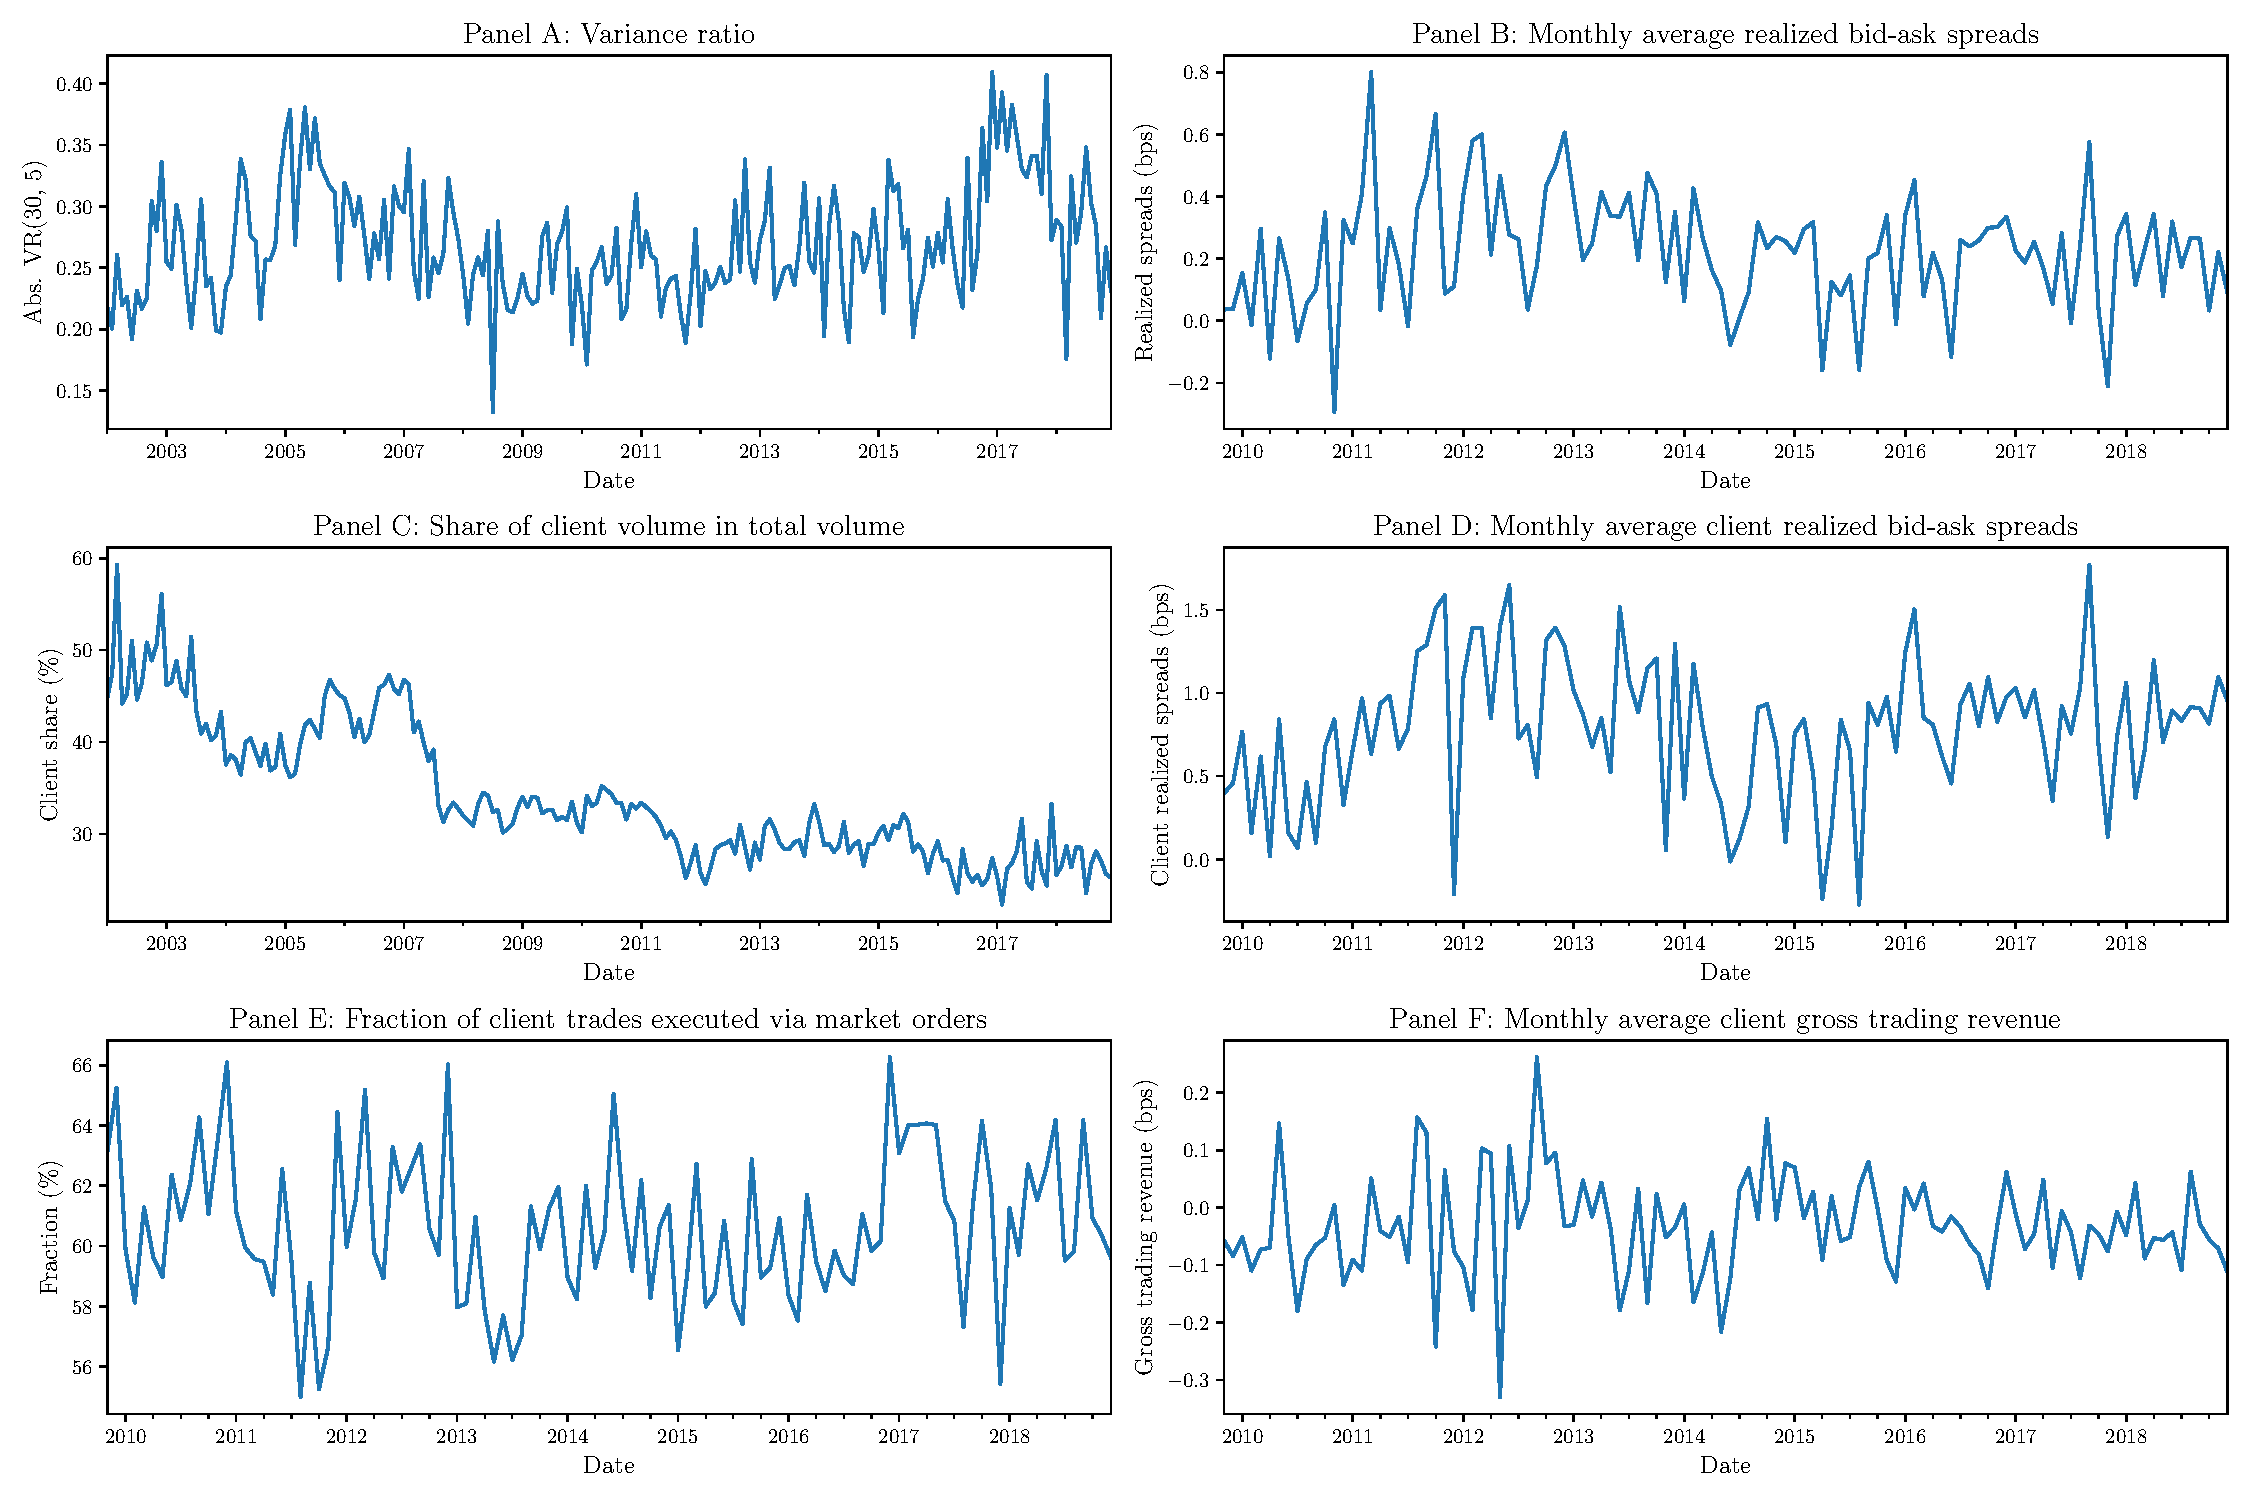
\includegraphics[width=0.9\linewidth]{Figures/Timeseries_monthly}
\label{fig:timeseriesmonthly}
\end{figure}


\end{document} 